%----------------------------------------------------------------------------------------
%    PACKAGES AND THEMES
%----------------------------------------------------------------------------------------

\documentclass[8pt, aspectratio=169]{beamer}
\usepackage{graphicx}
\usepackage{ragged2e}
\usetheme{Malmoe}
\usepackage{caption}
\setbeamercolor{background canvas}{bg=white}
\setbeamercolor{normal text}{fg=black}
\setbeamertemplate{footline}[frame number]
\addtobeamertemplate{footline}{\ifnum\value{framenumber}=1\else\hspace*{\fill}\fi}{}
\definecolor{LightCyan}{rgb}{0.87, 0.87, 0.87}
\setbeamercolor{section in toc}{fg=black}
\setbeamercolor{subsection in toc}{fg=black}
\setbeamertemplate{caption}[numbered]
\setbeamercolor{headline}{bg=white}
\setbeamercolor{title}{fg=black}
\setbeamercolor{frametitle}{bg=white, fg=black}
\usepackage{svg}
\usepackage[T2A]{fontenc}
\usepackage[utf8]{inputenc}
\usepackage[english,russian]{babel}
\usepackage{longtable}
\usepackage{hyphenat}
\setbeamertemplate{navigation symbols}{}
\usepackage{ragged2e}
\let\raggedright=\RaggedRight
\usepackage{colortbl}
\usepackage{xcolor}
\usepackage{tikz}
\usepackage{tabularx}
\hyphenation{тех-но-ло-гия}
\begin{document}
	\setbeamertemplate{frametitle}[default][center]
	
	%----------------------------------------------------------------------------------------
	%    TITLE PAGE
	%----------------------------------------------------------------------------------------
	
	\begin{frame}[noframenumbering,plain]
		\begin{columns}[T] % создаем две колонки
			% Первая колонка для логотипа
			\begin{column}{0.2\textwidth}
				
\includegraphics[width=2.5cm]{assets/b_logo.png} % Укажите путь к логотипу
			\end{column}
			% Вторая колонка для текста
			\begin{column}{0.8\textwidth}
				\centering
				{\footnotesize Министерство науки и высшего образования Российской Федерации\\
					
					Федеральное государственное автономное образовательное учреждение высшего образования\\
					
					<<Московский государственный технический университет
					имени Н.~Э.~Баумана
					(национальный исследовательский университет)>> \\
					
					(МГТУ им.~Н.~Э.~Баумана)} 
			\end{column}
		\end{columns}
		\vfill
		\centering
		{\LARGE \textbf{Метод построения синтаксических деревьев для ограниченного естественного русского языка на основе наиболее употребимых грамматик}} \\
		\vfill\vfill\vfill
		
		\raggedleft
		{\large Группа: ИУ7-84Б} \\
		
		{\large Студент: Бугаков Иван Сергеевич} \\
		
		{\large Научный руководитель: Строганов Юрий Владимирович} \\
		\vfill\vfill
		\centering
		{\small 2026 г.}
		
	\end{frame}
	
	\justifying  
	
	\setcounter{framenumber}{1}
	
	\begin{frame}{\centering Актуальность}
		\setlength{\parindent}{.5cm}
		В отечественной корпусной и прикладной лингвистике преобладающим формализмом в области синтаксического анализа являются системы зависимостей.
		
		В недавнем времени появились работы, посвященные альтернативным формализмам и их использованию в прикладной и корпусной лингвистике, например:
		\begin{itemize}
			\item[---] работы по созданию корпуса с синтаксической разметкой систем составляющих;
			\item[---] работы по созданию корпуса с разметкой систем синтаксических групп;
			\item[---] работы по созданию методов автоматического построения систем составляющих, на основе уже существующих разметок систем зависимостей.
		\end{itemize}
		
		Данные работы свидетельствуют о необходимости разработки автоматизированных методов построения систем составляющих для русского языка.
		
		Системы составляющих в прикладной и компьютерной лингвистике позволяют решать задачи:
		\begin{itemize}
			\item[---] генерации текстов;
			\item[---] автоматического реферирования текстов;
			\item[---] установления авторства текстов;
			\item[---] информационного поиска;
			\item[---] машинного перевода;
			\item[---] семантической разметки.
		\end{itemize}
		
%		Существуют, однако, альтернативные формализмы, такие как системы составляющих и системы синтаксических групп. Появление в недавнем времени работ, посвященных созданию корпусов с разметкой систем составляющих и систем синтаксических групп, а также разработке методов преобразования систем зависимостей в системы составляющих, свидетельствует о необходимости автоматизации построения данных видов синтаксических систем, как на основе исходных текстовых данных, так и уже существующих систем зависимостей.
		
%		Системы составляющих в прикладной и компьютерной могут быть использованы для решения задач генерации текстов, автоматического реферирования, установления авторства текстов, информационного поиска, машинного перевода, семантической разметки, а также для исследования синтаксических конструкций языка.
	\end{frame}
	
	\begin{frame}{\centering Цель и задачи работы}
		\setlength{\parindent}{.5cm}
		\textbf{Цель работы}~---~разработка метода построения синтаксических деревьев для ограниченного естественного русского языка на основе наиболее употребимых грамматик.\\
		
		\textbf{Задачи:}
		\begin{itemize}
			\item[---] проанализировать предметную область автоматизированного построения синтаксических деревьев ограниченного естественного русского языка;
			\item[---] провести сравнительный анализ существующих методов построения синтаксических деревьев и сформулировать требования к разрабатываемому методу;
			\item[---] формализовать постановку задачи в виде IDEF0-диаграммы;
			\item[---] разработать метод построения синтаксических деревьев ограниченного естественного русского языка;
			\item[---] обосновать выбор программных средств реализации и разработать программное обеспечение реализующее описанный метод;
			\item[---] определить зависимость времени построения синтаксических деревьев от количества словоформ в предложении, оценить точность и полноту разработанного метода.
			
		\end{itemize}
	\end{frame}

	\begin{frame}{\centering Системы зависимостей}
		\setlength{\parindent}{.5cm}
		Если \textit{П}~---~конечное линейное упорядоченное множество, то всякое дерево $D$, для которого \textit{П} служит множеством узлов, называется \textbf{деревом синтаксического подчинения (зависимостей) на \textit{П}}.
		
		\textbf{Размеченное дерево зависимостей}~---~ это упорядоченная четверка:
		$$
			\langle\textit{П},\rightarrow,Z,\psi\rangle,
		$$
		где 
		\begin{itemize}
			\item [---]
			$\langle\textit{П}, \rightarrow\rangle$~---~дерево зависимостей на $\textit{П}$;
			\item [---]	$Z$~---~конечное множество меток;
			\item [---]$\psi$~---~разметка, отображение множества дуг дерева в $Z$.
		\end{itemize}
		
		\begin{figure}[H]
			\centering
			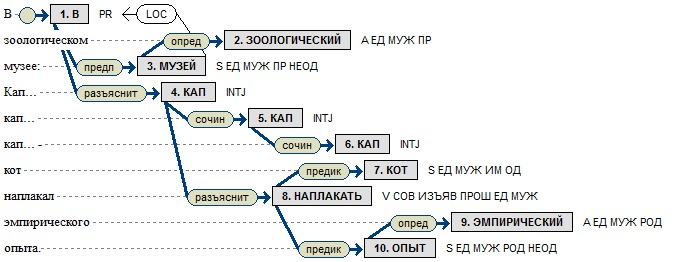
\includegraphics[width=0.75\linewidth]{assets/syntax_annotation.png}
		\end{figure}
	\end{frame}
	
	\begin{frame}{\centering Системы составляющих}
		\setlength{\parindent}{.5cm}
		Множество $C$ отрезков конечного линейно упорядоченного множества $\textit{П}$ называется \textbf{системой составляющих на $\textit{П}$}, если оно удовлетворяет следующим условиям:
		\begin{itemize}
			\item [---] $C$ содержит в качестве элементов само $\textit{П}$ и все элементы $\textit{П}$;
			\item[---] любые два отрезка из $C$ либо не пересекаются, либо один из них содержится в другом.
		\end{itemize}
		
		\textbf{Размеченная система составляющих}~---~упорядоченная тройка:
		$$
			\langle C,W,\varphi\rangle,
		$$
		где
		\begin{itemize}
			\item[---] $C$~---~система составляющих;
			\item[---] $W$~---~конечное множество меток;
			\item[---] $\varphi$~---~отображение $C$ в множество всех непустых подмножеств~$W$.
		\end{itemize}
		
		\begin{figure}[h!]
			\centering
			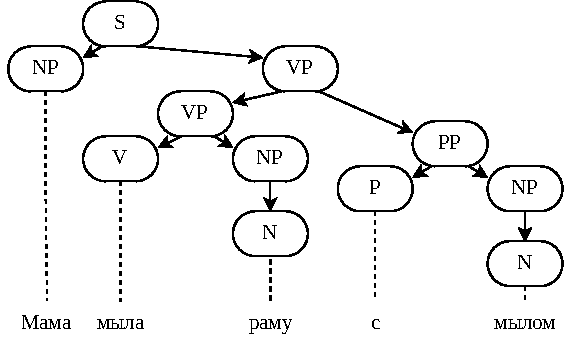
\includegraphics[height=0.4\textheight]{assets/marked_cons_tree.pdf}
		\end{figure}
		
	\end{frame}
	
	\begin{frame}{\centering Системы синтаксических групп}
		\setlength{\parindent}{.5cm}
		
		Пусть $C$~---~некоторое множество непустых подмножеств $\textit{П}$. \textbf{Синтаксическими группами (СГ)} называются элементы множества $C$.
		
		\textbf{Системой синтаксических групп} называется граф $\langle C,\rightarrow\rangle$, для которого выполняются следующие условия:
		\begin{itemize}
			\item[---] $C$ содержит $\textit{П}$ и все одноэлементные подмножества $\textit{П}$;
			\item[---] если $Е_1,\ E_2 \in C$ то либо $E_1 \cap E_2 = \varphi$, либо $E_1 \subseteq E_2$, либо $E_2 \subseteq E_1$;
			\item[---] если $E_1,\ E_2 \in C$, то $E_1$ и $E_2$ не зацепляются;
			\item[---] если $E_1 \rightarrow E_2$, то $E_1$ и $E_2$ непосредственно вложены в одну и ту же СГ;
			\item[---] СГ $E$ не может зависеть от самой себя;
			\item[---] если $E_1\rightarrow E_2$ и $E_2 \rightarrow E_1$, то $E_1 = E_2$;
			\item[---] если $E_1 \rightarrow E_2$ и $E$~---~произвольная СГ, то множества $E$ и $E_1 \cup E_2$ не зацепляются;
			\item[---] если $E_1 \rightarrow E_2$, $E_3 \rightarrow E_4$, то множества $E_1 \cup E_2$ и $E_3 \cup E_4$ не зацепляются.
		\end{itemize}
		
%		Размеченная система синтаксических групп~---~упорядоченная шестерка:
%		$$
%			\langle C,\rightarrow,W,Z,\varphi,\psi\rangle,
%		$$
%		где
%		\begin{itemize}
%			\item[---]$\langle C, \rightarrow\rangle$~---~система синтаксических групп;
%			\item[---]$W$~---~конечное множество меток СГ;
%			\item[---]$Z$~---~конечное множество меток при стрелках (типами синтаксических связей);
%			\item[---]$\varphi$~---~отображение $C$ в множество всех подмножеств $W$;
%			\item[---] $\psi$~---~отображение множества дуг графа $\langle C, \rightarrow \rangle$ в множество всех подмножеств $Z$.
%		\end{itemize}
		
		\begin{figure}[h!]
			\centering
			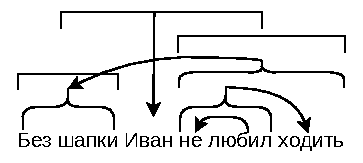
\includegraphics[width=0.4\textwidth]{assets/synt_group_tree.pdf}
		\end{figure}
		
	\end{frame}
	
	\begin{frame}{\centering Сравнение систем синтаксической разметки}
		\setlength{\parindent}{.5cm}
			\centering
			\begin{tabular}{|p{.39\textwidth}|p{.17\textwidth}|p{.17\textwidth}|p{.17\textwidth}|}
				\hline
				& Системы \newline зависимостей & \textbf{Системы \newline составляющих} & Системы \newline синтаксических групп\\\hline
				Выделение фразовых категорий & Нет & \textbf{Да}  & Да \\\hline
				Поддержка непроективных \newline предложений & Нет & \textbf{Да} &  Да \\\hline
				Возможность построения \newline нескольких деревьев разбора & Нет & \textbf{Да} & Да \\\hline
				Использование системы как \newline порождающей грамматики & Да & \textbf{Да} & Нет \\\hline
				Общедоступные корпуса с \newline разметкой таким видом систем & Да & \textbf{Да} & Нет \\\hline
			\end{tabular}
	\end{frame}
	
	\begin{frame}{\centering Алгоритмы построения систем составляющих}
		\setlength{\parindent}{.5cm}
		\begin{columns}[T]
			\begin{column}{0.5\linewidth}
				{\centering \textbf{Алгоритм Кока--Янгера--Касами (CYK)}\par}
				Два этапа:
				\begin{enumerate}
					\item построение таблицы составляющих;
					\item рекурсивное восстановление \mbox{деревьев} составляющих по полученной таблице.
				\end{enumerate}
				\begin{figure}[H]
					\centering
					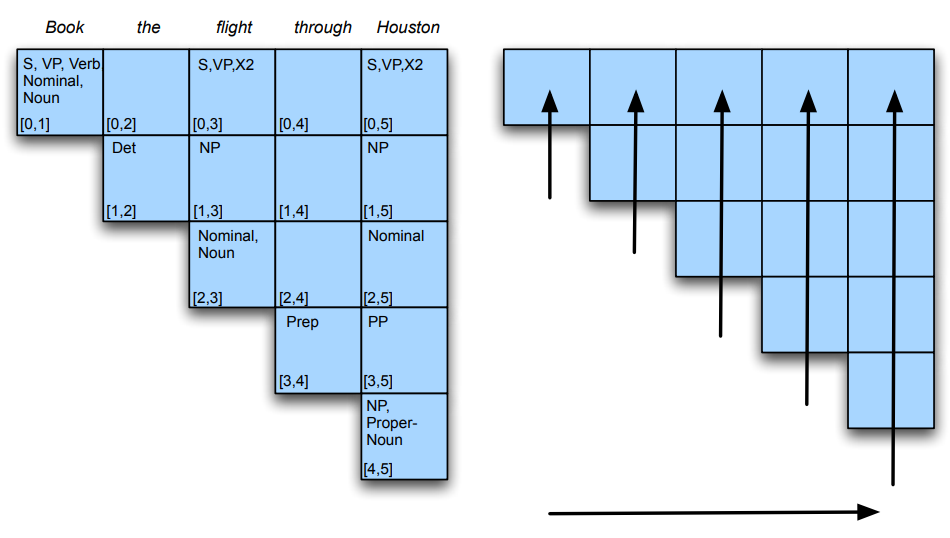
\includegraphics[width=0.75\linewidth]{assets/Cocke_DP_Algo.png}
				\end{figure}
				\begin{multline*}
					dp_{i,j} = dp_{i,j} \cup
					\{A \mid A \to B\,C \in P,\\ B \in dp_{i,k},\; C \in dp_{k,j}\}
				\end{multline*}
				
			\end{column}
			\begin{column}{0.5\linewidth}
				{\centering \textbf{Алгоритм Эрли}\par}
				Два этапа:
				\begin{enumerate}
					\item заполнение массива состояний \mbox{построенных} поддеревьев;
					\item рекурсивное восстановление \mbox{деревьев} составляющих по \mbox{заполненному} массиву.
				\end{enumerate}
%				Состояния описываются тройками:
%				$$
%				\langle r,\ p,\ [i,j]\rangle
%				$$
%				где
%				\begin{itemize}
%					\item[---]$r$~---~правило грамматики;
%					\item[---] $p \in \overline{0,m}$~---~позиция правиле $r$;
%					\item[---] $[i, j],\ 0\leqslant i\leqslant j \leqslant n$~---~границы фрагмента исходного предложения, соответствующие части правила $r$, до метки $p$. 
%				\end{itemize}
				Три используемые операции:
				\begin{itemize}
					\item[---] операция предсказания~---~добавление выводов из нетерминала в текущем состоянии;
					\item[---] операция чтения терминала~---~увеличение длины обработанного префикса при совпадении терминала в текущем состоянии с соответствующей словоформой входного предложения;
					\item[---] операция завершения разбора правила~---~замена разобранного в данном состоянии нетерминала на его разбор во всех других состояниях данной позиции.
				\end{itemize}
			\end{column}
		\end{columns}
	\end{frame}
	\begin{frame}{\centering Сравнение алгоритмов построения систем составляющих}
				\setlength{\parindent}{.5cm}
			\centering
			\begin{tabular}{|p{.63\textwidth}|p{.15\textwidth}|p{.15\textwidth}|}
				\hline
				Критерий & \textbf{Алгоритм CYK} & Алгоритм Эрли\\
				\hline
				Вычислительная сложность в худшем случае & \textbf{$O(n^3)$} & $O(n^3)$ \\
				\hline
				Требуется предварительное приведение к НФХ & \textbf{Да} & Нет\\
				\hline
				Максимальная длина правой части правила без преобразования & \textbf{2} & Не ограничена\\
				\hline
				Число параметров, определяющих разбор подотрезка предложения & \textbf{2} & 3\\
				\hline
				Число типов операций для построения составляющей & \textbf{1} & 3\\
				\hline
				Оценка числа состояний, худший случай & \textbf{$O(n^2|N|)$} & $O(n^3|P|)$\\
				\hline
				Оценка памяти в худшем случае & \textbf{$O(n^2)$} & $O(n^3)$ \\
				\hline
				Построение таблицы составляющих предложения & \textbf{Да} & Нет\\
				\hline
				Возможность вероятностного выбора синтаксической единицы для разрешения неоднозначности разбора & \textbf{Да} & Да\\
				\hline
			\end{tabular}
		\normalsize
	\end{frame}
	\begin{frame}{\centering Постановка задачи}
		\begin{figure}[h!]
			\centering
			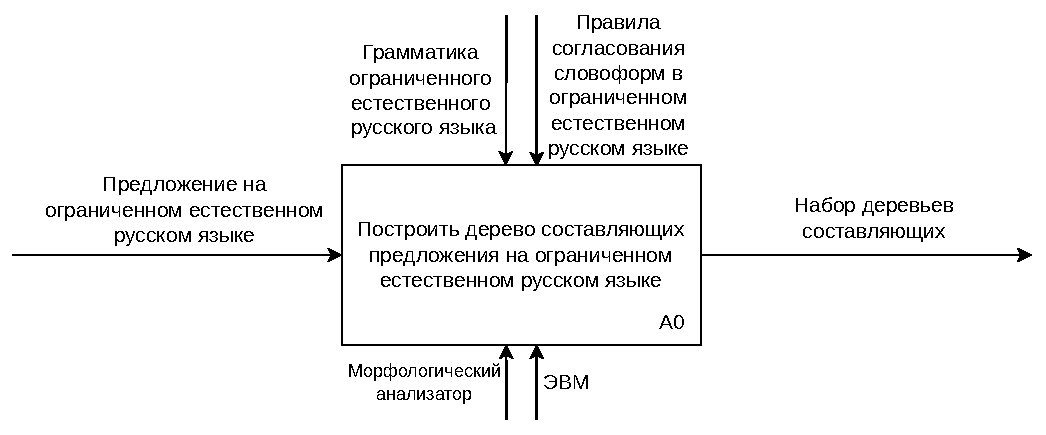
\includegraphics[width=\textwidth]{assets/A0.pdf}
		\end{figure}
	\end{frame}
	\begin{frame}{\centering Формальная модель метода}
		\begin{figure}[h!]
			\centering
			
\includegraphics[width=\textwidth]{assets/A1.pdf}
		\end{figure}
	\end{frame}
	\begin{frame}{\centering Алгоритм построения таблицы составляющих}
		\begin{figure}[h!]
			\centering
			
\includegraphics[height=0.9\textheight]{assets/cyk_scheme.pdf}
		\end{figure}
	\end{frame}
	\begin{frame}{\centering Восстановление деревьев составляющих}
		\begin{columns}[T]
			\begin{column}{0.5\linewidth}
				{\centering \textbf{Алгоритм восстановления деревьев составляющих}\par}
				\begin{figure}[h!]
					\centering
					
\includegraphics[width=\textwidth]{assets/tree_scheme_global.pdf}
				\end{figure}
			\end{column}
			\begin{column}{0.5\linewidth}
				{\centering \textbf{Алгоритм обработки унарных правил на отрезке длины 1}\par}
				\begin{figure}[h!]
					\centering
					
\includegraphics[height=0.8\textheight]{assets/tree_scheme_unary_1.pdf}
				\end{figure}
			\end{column}
		\end{columns}
	\end{frame}
	\begin{frame}{\centering Восстановление деревьев составляющих}
		\begin{columns}[T]
			\begin{column}{0.5\linewidth}
				{\centering \textbf{Алгоритм обработки бинарных правил}\par}
				\begin{figure}[h!]
					\centering
					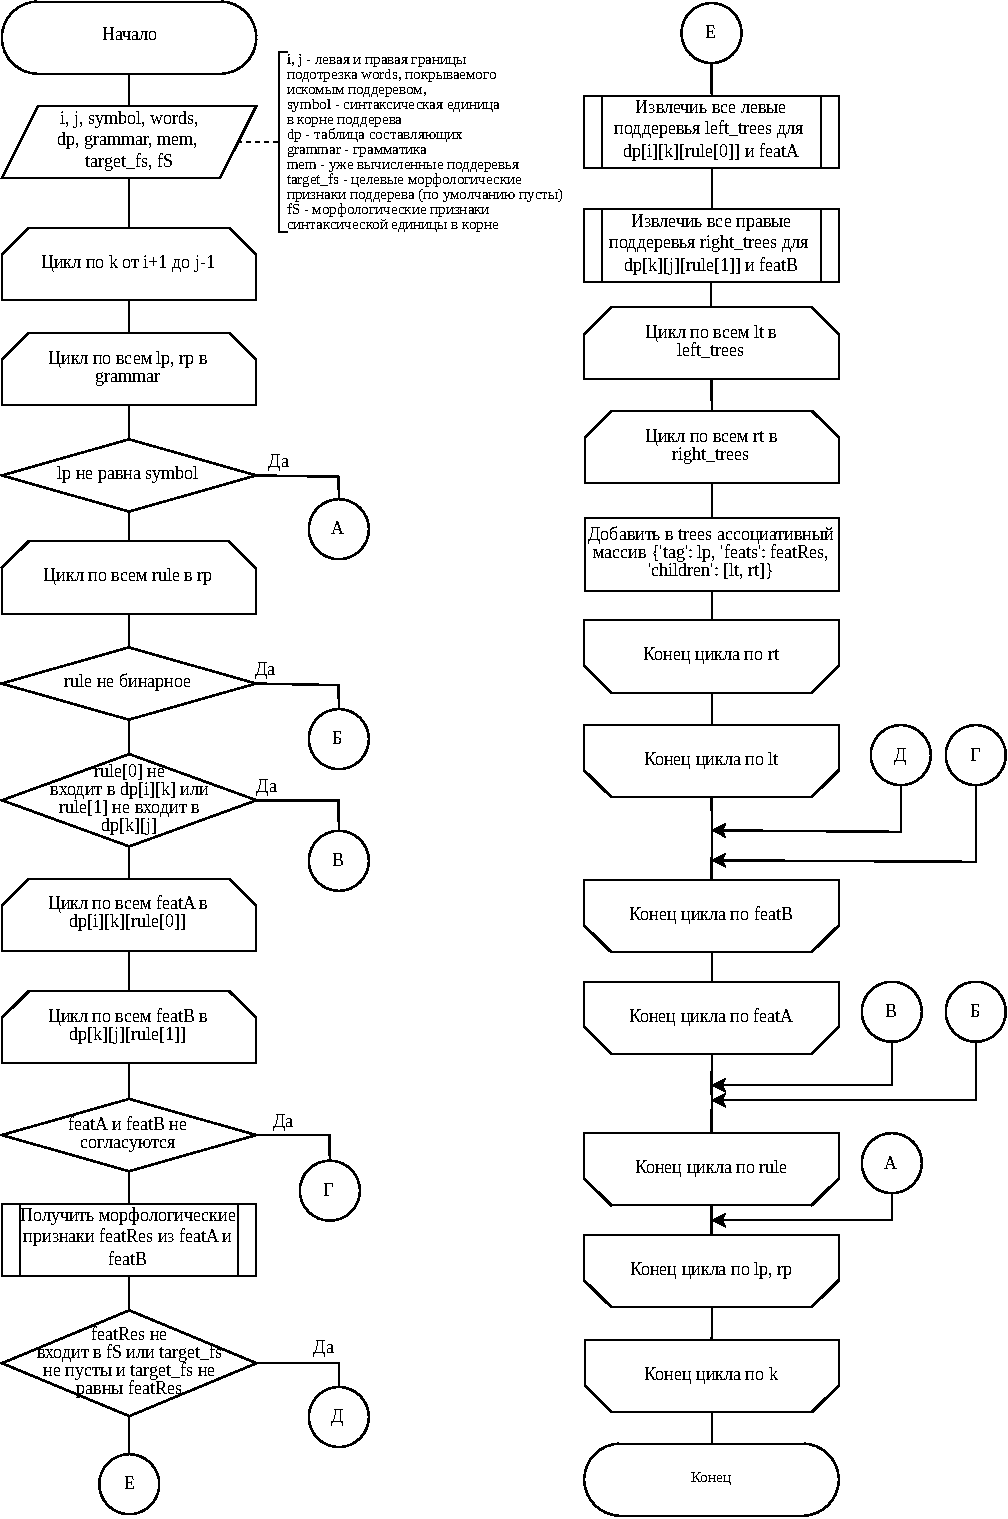
\includegraphics[height=\textwidth]{assets/tree_scheme_binary.pdf}
				\end{figure}
			\end{column}
			\begin{column}{0.5\linewidth}
				{\centering \textbf{Алгоритм обработки унарных правил на отрезке длины больше 1}\par}
				\begin{figure}[h!]
					\centering
					
\includegraphics[height=\textwidth]{assets/tree_scheme_unary_more_1.pdf}
				\end{figure}
			\end{column}
		\end{columns}
	\end{frame}
	\begin{frame}{\centering Реализация разработанной системы}
		\begin{columns}[T]
			\begin{column}{.4\linewidth}
				\begin{figure}[h!]
					\centering
					
\includegraphics[width=\linewidth]{assets/components.pdf}
				\end{figure}
			\end{column}
			\begin{column}{.65\linewidth}
				\setlength{\parindent}{.5cm}
				Выбранные языки и технологии:
				\begin{itemize}
					\item[---] Python~---~язык реализации разработанного метода и серверной составляющей web-приложения;
					\item[---] PyMorphy~---~используемый морфологический анализатор;
					\item[---] FastApi~---~фреймворк реализации серверной составляющей \mbox{web-приложения};
					\item[---] TypeScript~---~язык реализации клиентской составляющей \mbox{web-приложения};
					\item[---] React~---~фреймворк реализации клиентской составляющей \mbox{web-приложения};
					\item[---] PyTest~---~библиотека реализации модульного тестирования.
				\end{itemize}
				
				Покрытие строк кода по результатам модульного тестирования:
				\begin{itemize}
					\item[---] функции построения таблицы составляющих~---~$97.6\%$;
					\item[---] функций восстановления деревьев составляющих~---~$90.6\%$.
				\end{itemize}
			\end{column}
		\end{columns}
	\end{frame}
%	\begin{frame}{\centering Реализация и тестирование}
%		\normalsize
%		\setlength{\parindent}{.5cm}
%		Выбранные языки и технологии:
%		\begin{itemize}
%			\item[---] Python~---~язык реализации разработанного метода и серверной составляющей web-приложения;
%			\item[---] PyMorphy~---~используемый морфологический анализатор;
%			\item[---] FastApi~---~фреймворк реализации серверной составляющей web-приложения;
%			\item[---] TypeScript~---~язык реализации клиентской составляющей web-приложения;
%			\item[---] React~---~фреймворк реализации клиентской составляющей web-приложения
%			\item[---] PyTest~---~библиотека реализации модульного тестирования.
%		\end{itemize}
%		
%		Покрытие строк кода по результатам модульного тестирования:
%		\begin{itemize}
%			\item[---] функции построения таблицы составляющих~---~$97.6\%$;
%			\item[---] функций восстановления деревьев составляющих~---~$90.6\%$.
%		\end{itemize}
%		
%		
%	\end{frame}
	\begin{frame}{\centering Пример работы программы}
		\normalsize
		\setlength{\parindent}{.5cm}
		
		
		\begin{figure}[h!]
			\centering
			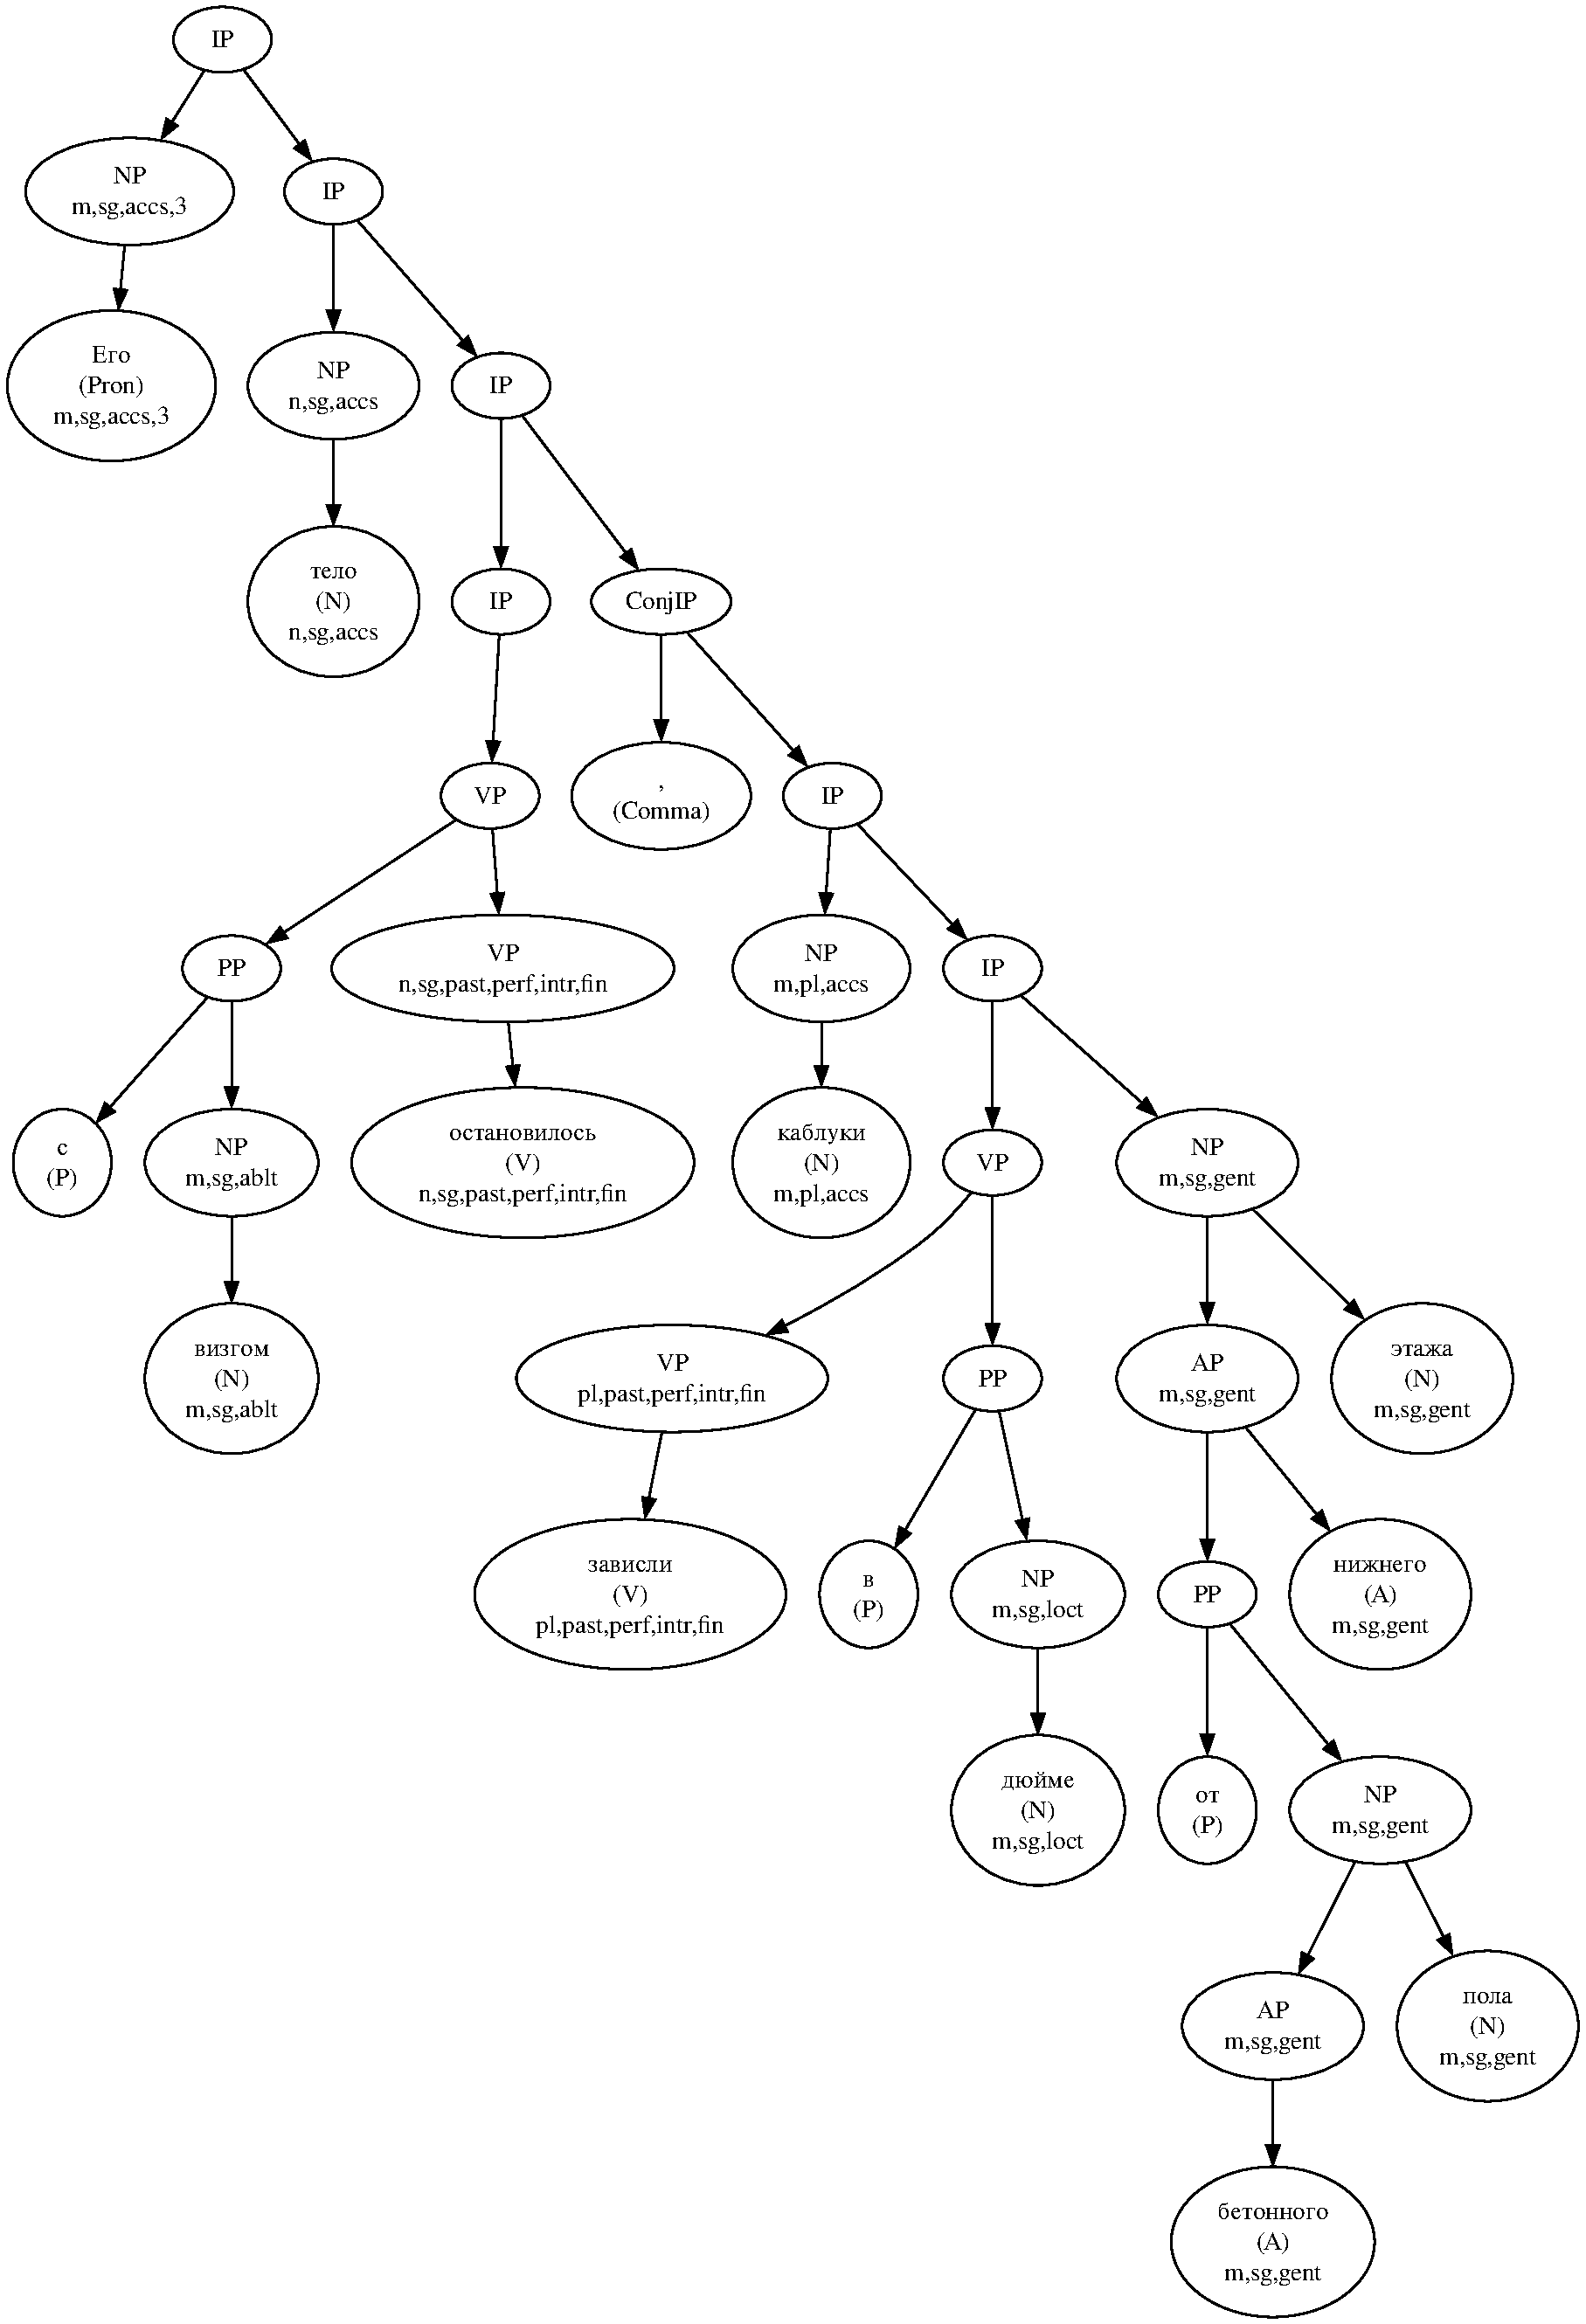
\includegraphics[height=.8\textheight]{assets/451_2.pdf}
		\end{figure}
		\vspace{-0.15cm}
		
		Дерево составляющих предложения: <<Его тело с визгом остановилось, каблуки зависли в дюйме от бетонного пола нижнего этажа.>>
	\end{frame}
	\begin{frame}{\centering Зависимость времени выполнения от числа словоформ}
		\normalsize
		\begin{columns}[T]
			\begin{column}{0.5\linewidth}
				\begin{figure}[h!]
					\centering
					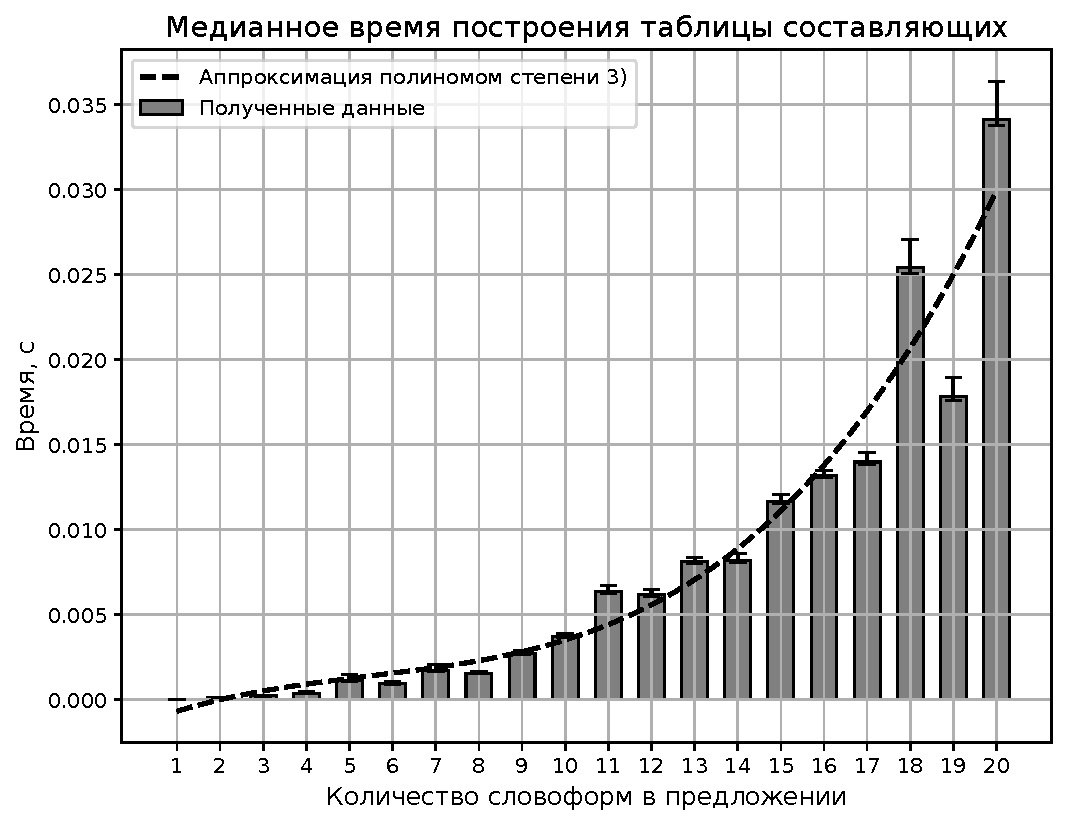
\includegraphics[width=\textwidth]{assets/benchmark_cyk_hist.pdf}
				\end{figure}
				\vspace{-0.3cm}
				
				Аппроксимация:
				\begin{multline*}
					T_{table}(n) \approx 7.85 \cdot 10^{-6} n^3 -1.29\cdot 10^{-4}n^2+1.01\cdot 10^{-3}n-\\-1.56\cdot 10^{-3}
				\end{multline*}
			\end{column}
			\begin{column}{0.5\linewidth}
				\begin{figure}[h!]
					\centering
					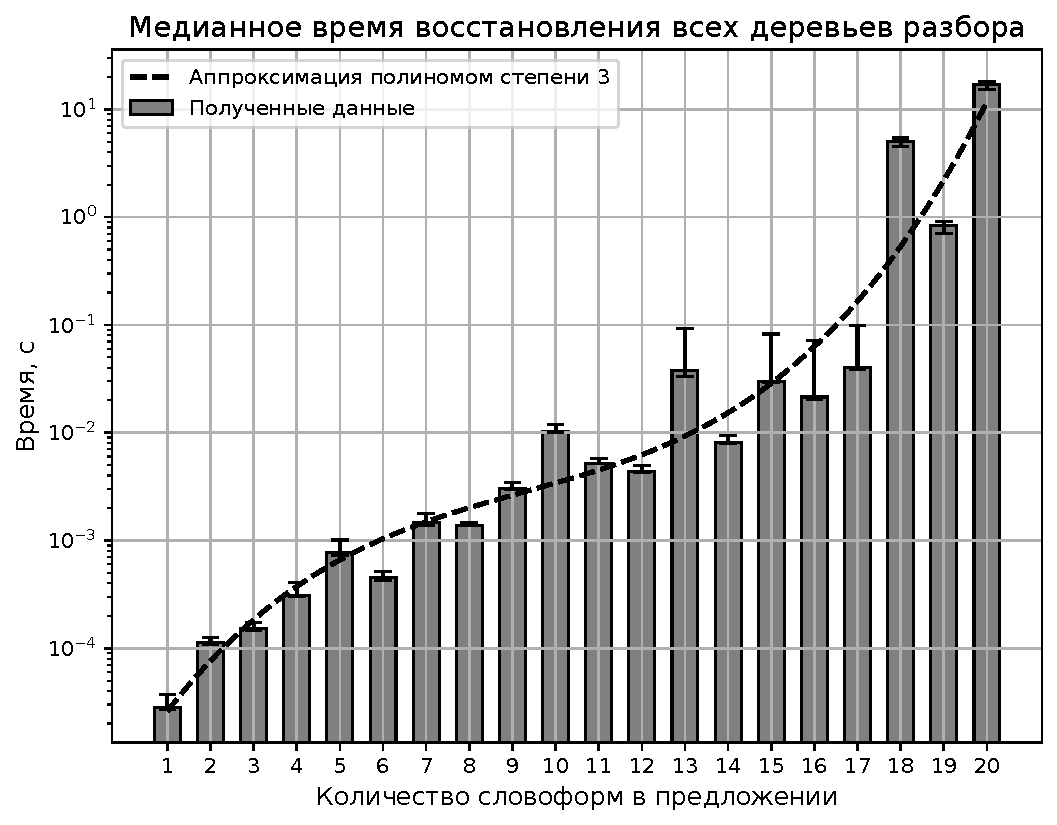
\includegraphics[width=\textwidth]{assets/benchmark_trees_total_log_hist.pdf}
				\end{figure}
				\vspace{-0.3cm}
				
				Аппроксимация:
				\begin{multline*}
					T_{tree}(n) \approx 4.52 \cdot 10^{-3} n^3 -1.26\cdot 10^{-1}n^2+1.42n-\\-11.86
				\end{multline*}
			\end{column}
		\end{columns}
	\end{frame}
	
	\begin{frame}{\centering Точность и полнота разработанного метода}
		\normalsize
		\setlength{\parindent}{.5cm}
		\begin{columns}[T]
			\begin{column}{0.5\linewidth}
				\centering\small
				\begin{tabular}{|p{0.4\textwidth}|p{0.5\textwidth}|}
					\hline
					Число словоформ в исходном предложении & Число восстановленных \newline деревьев составляющих\\\hline
					1 & 1\\\hline
					2 & 3 \\\hline
					3 & 2 \\\hline
					4 & 4 \\\hline
					5 & 16 \\\hline
					6 & 8 \\\hline
					7 & 96 \\\hline
					8 & 44 \\\hline
					9 & 268 \\\hline
					10 & 1436 \\\hline
					11 & 362 \\\hline
					12 & 480 \\\hline
					13 & 11032 \\\hline
					14 & 1600 \\\hline
					15 & 8748 \\\hline
					16 & 3362 \\\hline
					17 & 13374 \\\hline
					18 & 937755 \\\hline
					19 & 157544 \\\hline
					20 & 2776928 \\\hline
				\end{tabular}
				\normalsize
			\end{column}
			\begin{column}{0.5\linewidth}

				Полученные значения точности и полноты:
				\begin{itemize}
					\item[---] точность~---~$0.68$;
					\item[---] полнота~----~$0.71$;
					\item[---] F1-мера~---~$0.69$.
				\end{itemize}
				
				Сравнение с методами построения деревьев составляющих по готовым деревьям зависимостей:
					\centering
					\begin{tabular}{|p{0.3\linewidth}|p{0.15\linewidth}|p{0.15\linewidth}|p{0.15\linewidth}|}
						\hline
						Синтаксический\newline анализатор & Точность & Полнота & F1-мера\\\hline
						Stanza & 0.83 & 0.83 & 0.83 \\\hline
						SpaCy & 0.70 & 0.69 & 0.70 \\\hline
						\textbf{Разработанный метод} & \textbf{0.68} & \textbf{0.71} & \textbf{0.69}\\\hline
						Natasha & 0.68 & 0.49 & 0.57 \\\hline
					\end{tabular}
				
			\end{column}
		\end{columns}
	\end{frame}
	\begin{frame}{\centering Заключение}
		\setlength{\parindent}{.5cm}
			Цель работы~---~разработка метода построения синтаксических деревьев для ограниченного естественного русского языка на основе наиболее употребимых грамматик~---~была достигнута.
		
		В ходе выполнения выпускной квалификационной работы были выполнены следующие задачи:
		\begin{itemize}
			\item[---] проанализирована предметная область автоматизированного построения синтаксических деревьев ограниченного естественного русского языка;
			\item[---] проведен сравнительный анализ существующих методов построения синтаксических деревьев и сформулированы требования к разрабатываемому методу;
			\item[---] формализована постановка задачи в виде IDEF0-диаграммы;
			\item[---] разработан метод построения синтаксических деревьев ограниченного естественного русского языка;
			\item[---] обоснован выбор программных средств реализации и разработано программное обеспечение реализующее описанный метод;
			\item[---] определена зависимость времени построения синтаксических деревьев от количества словоформ в предложении, оценена точность и полнота разработанного метода.
		\end{itemize}
		
	\end{frame}
	\begin{frame}{\centering Дальнейшее развитие}
		
		Дальнейшее развитие может быть достигнуто за счет:
		\begin{itemize}
			\item[---] более высокой <<детализации>> используемой грамматики, выделения подъединиц текущих синтаксических единиц, ввода новых правил грамматики;
			\item[---] использования более подробного морфологического анализатора, охватывающего все существующие в языке части речи и их морфологические характеристики;
			\item[---] внедрения возможности автоматического разрешения неоднозначности среди всех возвращаемых методом деревьев составляющих;
			\item[---] оптимизации временных затрат этапа восстановления деревьев составляющих.
		\end{itemize}
	\end{frame}
	
	
\end{document}